\documentclass[journal]{IEEEtran}
\usepackage{amsmath,amssymb,amsfonts}
\usepackage{algorithmic}
\usepackage{algorithm}
\usepackage{graphicx}
\usepackage{textcomp}
\usepackage{xcolor}
\usepackage{booktabs}
\usepackage{multirow}
\usepackage{tikz}
\usetikzlibrary{shapes,arrows,positioning,fit,calc}
\usepackage{listings}
\usepackage{url}

\lstset{
  basicstyle=\ttfamily\footnotesize,
  breaklines=true,
  frame=single,
  numbers=left,
  numberstyle=\tiny,
  captionpos=b
}

\begin{document}

\title{Design, Implementation, and Evaluation of the BitMLx Toolchain for Cross-Chain Smart Contracts on UTXO-Based Blockchains}

\author{Ngo~Vinh~Huy,~Nguyen~Gia~Linh,~and~Tran~Tuan~Dung%
\thanks{The authors are with the University of Information Technology, Vietnam National University Ho Chi Minh City, Vietnam.}%
\thanks{Source code and reproducible artifacts: \protect\url{https://github.com/sampleit533/BitMLx/}.}}

\maketitle

\begin{abstract}
Cross-chain smart contracts that simultaneously govern assets on multiple UTXO-based blockchains present significant security and engineering challenges. Existing approaches, such as hash time-locked contracts, address only simple atomic swaps and do not provide a general implementation framework for multi-party protocols with formally specified branching behavior. This article presents the design, implementation, and evaluation of a BitMLx-based toolchain that compiles a single high-level cross-chain contract specification into paired BitML contracts for Bitcoin and Dogecoin, and then into UTXO-level Balzac transaction artifacts. The repository integrates a Haskell BitMLx compiler, the Racket BitML compiler, Docker-based reproducible execution scripts, a pytest integration test suite, pre-built artifacts, and a Flask web interface for inspecting and experimenting with contracts. We redeployed the system on the evaluation machine, rebuilt the Docker image with host networking, reran the integration tests, and validated the web interface including a live template compilation request. We analyze the compiler architecture directly from the source code, emphasizing priority choice compilation, step-secret generation, stipulation/refund wrapping, collateral accounting, and well-formedness checks. The system is evaluated on four representative applications: ReceiverChosenDenomination, TwoPartyAgreement, MultichainPaymentExchange, and MultichainLoanMediator. The generated artifacts contain 51, 51, 207, and 4,098 transactions per chain, with execution-tree depths of 6, 6, 9, and 27, respectively. The Bitcoin and Dogecoin outputs are structurally symmetric in all evaluated cases, while the randomized hash-replacement step intentionally changes concrete hash literals between runs. These results demonstrate the feasibility of an end-to-end BitMLx toolchain and highlight the principal trade-off of the approach: formal cross-chain expressiveness is obtained at the cost of substantial transaction expansion for deeply nested protocols.
\end{abstract}

\begin{IEEEkeywords}
Cross-chain smart contracts, BitMLx, BitML, UTXO, blockchain interoperability, domain-specific languages, formal methods
\end{IEEEkeywords}

\section{Introduction}

Digital assets increasingly span multiple blockchain networks, creating demand for smart contracts that coordinate actions across heterogeneous ledgers~\cite{bonneau2015sok,nakamoto2008bitcoin}. A user holding Bitcoin may wish to exchange assets with a counterparty on Dogecoin, or a decentralized lending protocol may require synchronized state transitions on two independent chains. These cross-chain interactions introduce fundamental challenges: transactions on one blockchain carry no inherent guarantee of corresponding execution on another, and a malicious participant may exploit this asynchrony to gain unilateral advantage~\cite{zamyatin2021sok}.

Current cross-chain solutions predominantly rely on hash time-locked contracts (HTLCs), which support only pairwise atomic swaps with limited expressiveness~\cite{herlihy2018atomic}. Bridge protocols offer broader interoperability but introduce additional validator, relayer, or custody assumptions, and bridge failures have repeatedly shown that such assumptions become high-value attack surfaces~\cite{belchior2021survey,zamyatin2021sok}. Neither approach provides a systematic framework for specifying, compiling, and testing arbitrary multi-party cross-chain contracts over independent UTXO ledgers.

BitMLx addresses this gap by extending the BitML smart contract language to the cross-chain setting~\cite{engel2025bitmlx}. While BitML enables formal specification and compilation of contracts for a single UTXO-based blockchain~\cite{bartoletti2018bitml}, BitMLx introduces priority choice operators and step secret mechanisms that ensure safe replication across two chains. From a single BitMLx specification, the compiler generates synchronized BitML contracts for each target blockchain, along with honest participant strategies that guarantee no honest party loses funds regardless of adversarial behavior.

Despite the theoretical elegance of BitMLx, no comprehensive implementation and evaluation of its compilation toolchain has been reported. The original BitMLx paper provides the formal foundations but does not address practical concerns such as automated build environments, end-to-end testing, artifact management, or interactive visualization of compiled contracts.

The main contributions of this article are as follows:
\begin{enumerate}
\item We document and systematize a complete BitMLx/BitML toolchain that compiles BitMLx specifications into UTXO-level transaction artifacts for Bitcoin and Dogecoin, integrating the Haskell-based BitMLx compiler with the Racket-based BitML compiler through Docker and shell automation.
\item We analyze the implementation at module level, including the embedded Haskell DSL, two-pass coin selection, stipulation contract, priority-choice compilation, step-secret naming scheme, collateral computation, and well-formedness validation.
\item We describe an integration testing framework that validates the end-to-end pipeline across four representative cross-chain applications by checking artifact existence, transaction counts, and execution tree depths.
\item We present the Flask-based artifact viewer and template-driven contract editor, explaining how it exposes compiled artifacts and safely generates user-modified Haskell examples for Docker-based compilation.
\item We evaluate the generated artifacts in terms of participant count, step-secret count, transaction count, tree depth, timeout horizon, and file size, thereby characterizing the practical overhead of the BitMLx compilation approach.
\end{enumerate}

The remainder of this article is organized as follows. Section~II reviews related work on cross-chain smart contracts and formal specification languages. Section~III presents the theoretical foundations of BitML and BitMLx. Section~IV describes the architecture and implementation of the toolchain. Section~V presents the four cross-chain applications used for evaluation. Section~VI reports the experimental results. Section~VII discusses the findings and limitations. Section~VIII concludes the article.

\section{Related Work}

\subsection{Cross-Chain Interoperability Mechanisms}

Cross-chain interoperability has been addressed through several distinct approaches, each with different trust assumptions and expressiveness.

Hash time-locked contracts represent the earliest trustless cross-chain mechanism. Herlihy~\cite{herlihy2018atomic} proposed the foundational framework for atomic cross-chain swaps using HTLCs, demonstrating their correctness under synchrony assumptions. Subsequent work by Thyagarajan et al.~\cite{thyagarajan2022universal} introduced verifiable timed signatures to reduce the on-chain footprint of atomic swaps. Han et al.~\cite{han2019threshold} proposed threshold signature-based protocols that eliminate the hash preimage revelation step. While these approaches provide atomicity guarantees, they support only simple two-party exchanges and cannot express multi-step protocols involving conditional logic, secret-based branching, or mediated dispute resolution.

Bridge protocols, including Cosmos IBC~\cite{kwon2019cosmos}, Polkadot XCMP~\cite{wood2016polkadot}, and various Ethereum-compatible bridges~\cite{wood2014ethereum}, enable general message passing between chains. Xie et al.~\cite{xie2022bridge} designed zkBridge for trustless cross-chain communication. Belchior et al.~\cite{belchior2021survey} provided a comprehensive survey of blockchain interoperability, classifying approaches by their trust model and communication pattern. However, bridges rely on external validators or relayers, introducing trust assumptions that have been exploited in high-profile attacks on bridge infrastructures.

Sidechain and relay chain architectures, as implemented by Polkadot~\cite{wood2016polkadot} and Cosmos~\cite{kwon2019cosmos}, provide shared security models but require participating chains to adopt specific consensus mechanisms. Layer-two protocols~\cite{gudgeon2020defi} offer scalability but similarly do not address interoperability between existing independent chains such as Bitcoin and Dogecoin.

\subsection{Smart Contract Specification Languages}

BitML, introduced by Bartoletti and Zunino~\cite{bartoletti2018bitml}, provides a process-algebraic language for specifying Bitcoin smart contracts with formal security guarantees. The BitML compiler translates high-level specifications into standard Bitcoin transactions~\cite{atzei2019developing}, and its computational soundness ensures that security properties verified at the symbolic level carry over to the computational execution. A model checker enables automated verification of contract liquidity, ensuring that funds are never permanently frozen~\cite{bartoletti2019bitml}.

Solidity and Vyper serve as the primary smart contract languages for Ethereum~\cite{wood2014ethereum} and EVM-compatible chains but operate within the account-based model and lack formal verification guarantees by default~\cite{tikhomirov2018smartcheck}. Move, developed for the Aptos and Sui blockchains~\cite{amsden2020move}, incorporates resource-oriented type systems that prevent common vulnerabilities, but targets a single-chain execution environment. Scilla, designed for the Zilliqa blockchain~\cite{sergey2019scilla}, uses an intermediate-level language amenable to formal verification but similarly addresses only single-chain execution. A recent comparative analysis by Bartoletti~\cite{bartoletti2025comparison} classifies these languages by expressiveness and verification support.

\subsection{Cross-Chain Smart Contract Languages}

BitMLx, proposed by Engel and Maffei~\cite{engel2025bitmlx}, extends BitML to support cross-chain contracts on UTXO-based blockchains. The language introduces priority choice operators and a compilation scheme that generates synchronized BitML contracts for two target chains. The formal security analysis demonstrates that honest participants following the prescribed strategy are guaranteed outcomes at least as favorable as in the ideal single-chain execution. The theoretical foundations are rigorous, with complete proofs of computational soundness and security.

To the best of our knowledge, no prior work has reported a complete implementation and empirical evaluation of the BitMLx compilation toolchain, including automated testing, artifact management, and interactive visualization capabilities.

\begin{table}[t]
\caption{Comparison of cross-chain smart contract approaches.}
\label{tab:comparison}
\centering
\footnotesize
\begin{tabular}{lccccc}
\toprule
Approach & \begin{tabular}[c]{@{}c@{}}Multi-\\party\end{tabular} & \begin{tabular}[c]{@{}c@{}}Formal\\guarantees\end{tabular} & \begin{tabular}[c]{@{}c@{}}UTXO\\support\end{tabular} & \begin{tabular}[c]{@{}c@{}}Complex\\logic\end{tabular} & \begin{tabular}[c]{@{}c@{}}Tool-\\chain\end{tabular} \\
\midrule
HTLC swaps & Limited & Partial & Yes & No & No \\
Bridge protocols & Yes & No & Limited & Yes & Partial \\
Relay chains & Yes & Partial & No & Yes & Yes \\
BitML & No & Yes & Yes & Yes & Yes \\
BitMLx (theory) & Yes & Yes & Yes & Yes & No \\
This work & Yes & Yes & Yes & Yes & Yes \\
\bottomrule
\end{tabular}
\end{table}

Table~\ref{tab:comparison} summarizes the comparison. Our work is the first to combine formal cross-chain guarantees with a complete, tested toolchain supporting UTXO-based blockchains.

\section{Theoretical Foundations}

\subsection{UTXO Transaction Model}

Bitcoin-style blockchains employ the Unspent Transaction Output (UTXO) model, where funds are represented as discrete, unspent outputs of previous transactions rather than as account balances. Each UTXO is associated with spending conditions encoded in a scripting language. Common conditions include requiring a digital signature from a specified public key, revealing the preimage of a hash value, or waiting until a specified block height or timestamp.

A transaction consumes one or more UTXOs as inputs and produces new UTXOs as outputs. The total value of outputs must not exceed the total value of inputs, with the difference constituting the transaction fee. Smart contracts on UTXO-based blockchains are realized as interconnected sets of pre-signed transactions with carefully constructed spending conditions, rather than as persistent programs executing on a virtual machine.

\subsection{BitML: Single-Chain Contract Specification}

BitML provides a high-level language for specifying smart contracts on Bitcoin. A BitML contract $C$ is defined by a set of preconditions $G$ and a contract body. Preconditions specify the deposits each participant must commit and any secrets they must provide hash commitments for. The contract body is composed from the following primitives:

\begin{itemize}
\item $\textsf{withdraw}~A$: transfer the contract balance to participant $A$.
\item $\textsf{split}~[(v_1, C_1), \ldots, (v_n, C_n)]$: divide the balance among sub-contracts.
\item $A : C$: require authorization from participant $A$ to proceed with $C$.
\item $\textsf{reveal}~\vec{s}~.~C$: require revelation of secrets $\vec{s}$ before executing $C$.
\item $\textsf{after}~t : C$: enable $C$ only after time $t$.
\item $C_1 + C_2$: offer a choice between $C_1$ and $C_2$.
\end{itemize}

The BitML compiler translates these specifications into standard Bitcoin transactions, and a model checker verifies properties such as liquidity.

\subsection{BitMLx: Cross-Chain Extension}

BitMLx extends BitML to the cross-chain setting by introducing the priority choice operator and associated compilation mechanisms. A BitMLx contract operates over two blockchains simultaneously, with deposits specified as pairs $(v_B, v_D)$ representing values on Bitcoin and Dogecoin, respectively.

\subsubsection{Priority Choice}

The priority choice operator $D +\!\!> C$ specifies that guarded contract $D$ has higher execution priority than contract $C$. The semantics ensure that participants first attempt to execute $D$ on both chains; only if $D$ is not executed within the allotted time window does $C$ become available. This mechanism is fundamental to preventing the situation where a participant executes a favorable branch on one chain while the unfavorable fallback executes on the other.

\subsubsection{Step Secrets}

Each participant holds step secrets corresponding to each node in the contract execution tree. When a participant executes a priority choice branch, they must reveal the corresponding step secret. This revelation serves as verifiable evidence of the action taken, enabling the compensation mechanism if the action is not replicated on the other chain.

\subsubsection{Compensation Phase}

If a participant executes a priority choice on one chain but fails to replicate the action on the other, honest participants can enter a compensation phase. By presenting the revealed step secret as evidence of the unilateral action, the honest participant can claim the full contract balance on the chain where the action was not replicated, ensuring they are at least as well off as in the ideal synchronized execution.

\subsubsection{Collateral}

To fund the compensation mechanism in multi-party contracts, each participant locks additional collateral proportional to the number of participants. For $n$ participants with total contract balance $b$, each participant contributes $(n-2) \times b$ in collateral.

\subsubsection{Compilation}

The BitMLx compiler $\mathcal{C}$ takes a BitMLx contract advertisement and produces a pair of BitML contract advertisements:
\begin{equation}
\mathcal{C}(\mathit{CA}^x) = (\mathit{CA}^B, \mathit{CA}^D)
\end{equation}
where $\mathit{CA}^B$ targets Bitcoin and $\mathit{CA}^D$ targets Dogecoin. The same compilation logic is applied twice with different coin selection functions: $\mathit{fst}$ for Bitcoin and $\mathit{snd}$ for Dogecoin. Table~\ref{tab:notation} summarizes the notation used throughout this article.

\begin{table}[t]
\caption{Summary of notation.}
\label{tab:notation}
\centering
\footnotesize
\begin{tabular}{cl}
\toprule
Symbol & Description \\
\midrule
$\mathcal{C}$ & BitMLx compiler function \\
$CA^x$ & BitMLx contract advertisement \\
$CA^B, CA^D$ & BitML advertisements for Bitcoin, Dogecoin \\
$D +\!\!> C$ & Priority choice: $D$ over $C$ \\
$n$ & Number of participants \\
$b$ & Total contract balance per chain \\
$T$ & Number of generated transactions \\
$d$ & Execution tree depth \\
$S$ & Number of step secrets \\
$t_{\max}$ & Maximum protocol timeout horizon \\
\bottomrule
\end{tabular}
\end{table}

% Part 2: Sections IV-VIII + Bibliography

\section{Toolchain Architecture and Implementation}

The toolchain is organized as four cooperating layers built around a shared artifact store: (i) a Haskell \emph{compiler layer} that lowers a single cross-chain specification into a pair of single-chain BitML programs; (ii) a Dockerized \emph{pipeline layer} that expands these programs into UTXO-level transaction artifacts; (iii) a \emph{testing layer} that asserts structural metrics over the generated artifacts; and (iv) a Flask \emph{web layer} that exposes the artifacts and supports interactive recompilation of user-modified templates. Fig.~\ref{fig:architecture} depicts this layered architecture and the data flow between layers.

\begin{figure*}[t]
\centering
\resizebox{0.86\textwidth}{!}{%
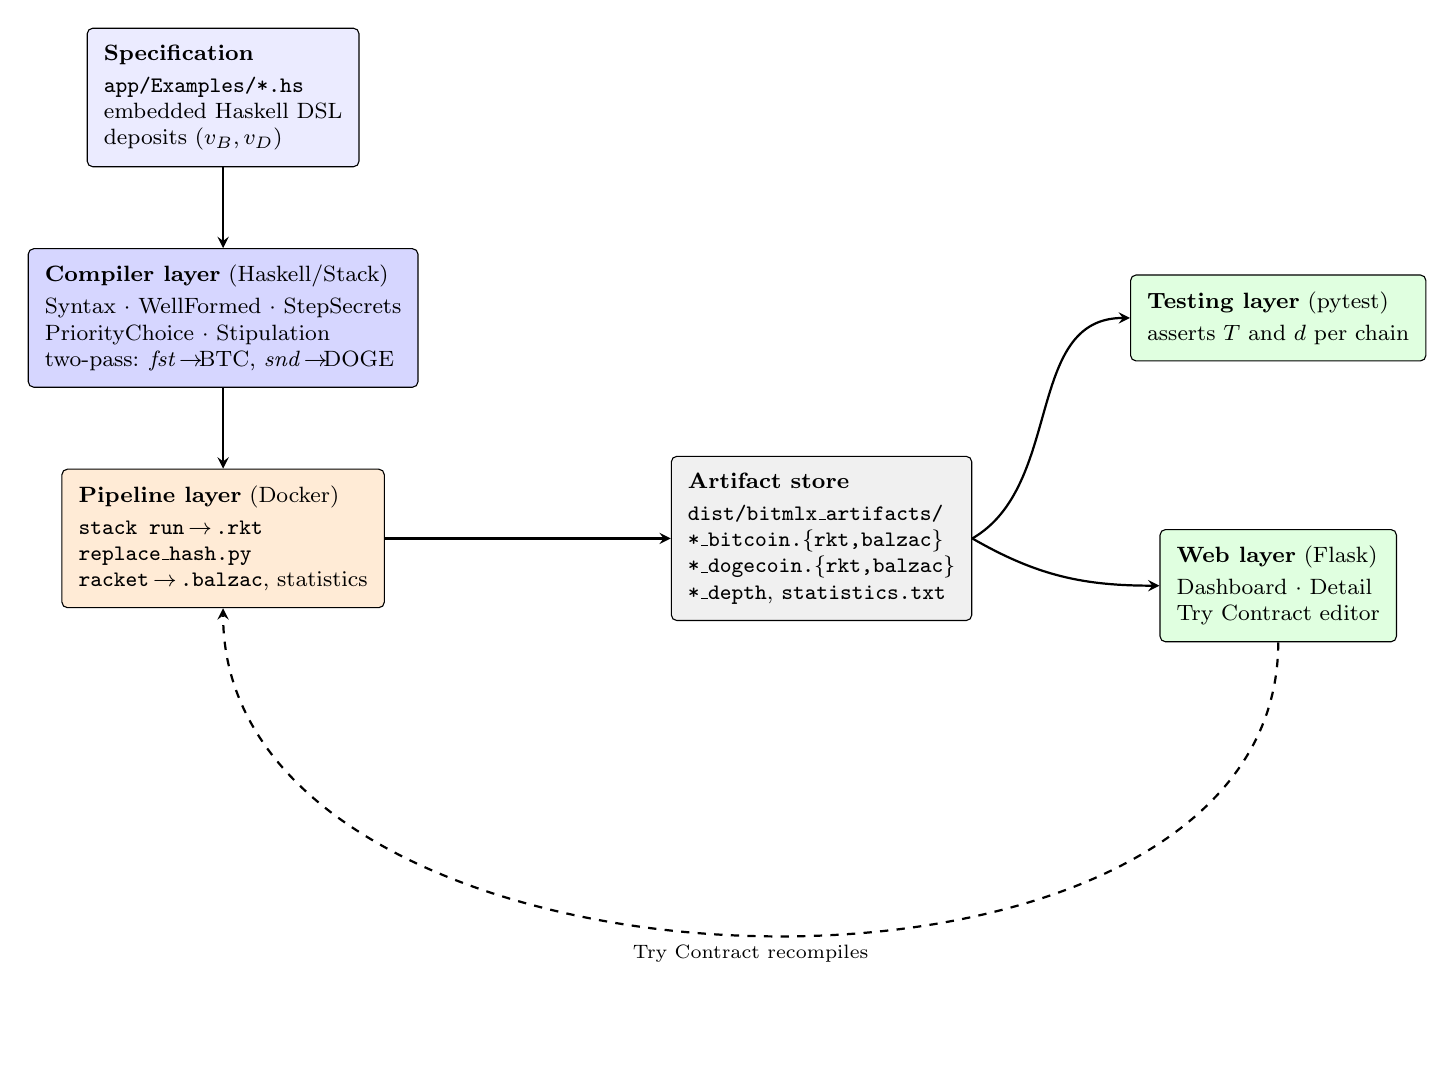
\begin{tikzpicture}[
    font=\footnotesize,
    >=stealth,
    box/.style={rectangle, draw, rounded corners=2pt, align=left, inner sep=6pt},
    arr/.style={->, thick},
    darr/.style={->, thick, dashed}
]
% Producer chain (left, top-down). No fixed text width: each box auto-sizes
% to its widest line so monospace tokens never overflow the border.
\node[box, fill=blue!8]    (src)  at (0,7.2)
     {\textbf{Specification}\\[2pt]\texttt{app/Examples/*.hs}\\ embedded Haskell DSL\\ deposits $(v_B,v_D)$};
\node[box, fill=blue!16]   (comp) at (0,4.4)
     {\textbf{Compiler layer} (Haskell/Stack)\\[2pt] Syntax $\cdot$ WellFormed $\cdot$ StepSecrets\\ PriorityChoice $\cdot$ Stipulation\\ two-pass: $\mathit{fst}\!\to\!$BTC, $\mathit{snd}\!\to\!$DOGE};
\node[box, fill=orange!16] (pipe) at (0,1.6)
     {\textbf{Pipeline layer} (Docker)\\[2pt] \texttt{stack run}\,$\to$\,\texttt{.rkt}\\ \texttt{replace\_hash.py}\\ \texttt{racket}\,$\to$\,\texttt{.balzac}, statistics};
% Artifact store (center)
\node[box, fill=gray!12]   (store) at (7.6,1.6)
     {\textbf{Artifact store}\\[2pt] \texttt{dist/bitmlx\_artifacts/}\\ \texttt{*\_bitcoin.\{rkt,balzac\}}\\ \texttt{*\_dogecoin.\{rkt,balzac\}}\\ \texttt{*\_depth}, \texttt{statistics.txt}};
% Consumers (right)
\node[box, fill=green!12]  (test) at (13.4,4.4)
     {\textbf{Testing layer} (pytest)\\[2pt] asserts $T$ and $d$ per chain};
\node[box, fill=green!12]  (web)  at (13.4,1.0)
     {\textbf{Web layer} (Flask)\\[2pt] Dashboard $\cdot$ Detail\\ Try Contract editor};
% Edges
\draw[arr] (src)  -- (comp);
\draw[arr] (comp) -- (pipe);
\draw[arr] (pipe) -- (store);
\draw[arr] (store.east) to[out=30,in=180]  (test.west);
\draw[arr] (store.east) to[out=-30,in=180] (web.west);
\draw[darr] (web.south) to[out=-90,in=-90]
      node[below, font=\scriptsize] {Try Contract recompiles} (pipe.south);
\end{tikzpicture}%
}
\caption{Layered architecture of the BitMLx toolchain. The Haskell compiler layer lowers a single cross-chain specification into paired single-chain BitML programs; the Dockerized pipeline layer expands them into UTXO-level Balzac artifacts; and the resulting artifact store is consumed by the pytest testing layer and the Flask web layer. The dashed edge denotes the interactive \emph{Try Contract} path, which re-enters the pipeline to compile user-modified templates.}
\label{fig:architecture}
\end{figure*}


\subsection{Technology Stack and Runtime Environment}

The implementation combines several technologies, each selected for a specific layer of the system rather than for incidental convenience. Table~\ref{tab:techstack} summarizes the stack observed during the redeployment on the evaluation machine.

\begin{table}[t]
\caption{Technology stack validated during local redeployment.}
\label{tab:techstack}
\centering
\footnotesize
\begin{tabular}{p{0.22\linewidth}p{0.31\linewidth}p{0.37\linewidth}}
\toprule
Layer & Technology & Role in the system \\
\midrule
Container runtime & Docker 29.4.2 & Reproducible Linux execution boundary \\
Base OS & Debian Bookworm & Package source for Racket, Python, LLVM, C toolchain \\
Haskell build & Stack 2.15.7, GHC 8.10.7 & Build and run the BitMLx compiler \\
BitML backend & Racket 8.7 & Execute \texttt{\#lang bitml} contracts \\
Auxiliary scripts & Python 3.11.2 & Hash replacement, statistics, pytest pipeline \\
Testing & pytest 9.0.3 & End-to-end regression tests \\
Web interface & Flask 3.1.3, Werkzeug 3.1.8 & Artifact dashboard and Try Contract API \\
Orchestration & Make 4.3, Bash & Local commands and Docker entry points \\
\bottomrule
\end{tabular}
\end{table}

The Haskell/Racket split is important architecturally. Haskell hosts the embedded BitMLx DSL and the source-to-source compiler that maps cross-chain abstractions to two single-chain BitML advertisements. Racket is then used as the execution environment for the existing BitML compiler, which expands the generated \texttt{.rkt} programs into Balzac transaction artifacts. Python does not participate in the core semantics; instead, it provides operational glue: replacing placeholder hashes, parsing statistics, driving pytest assertions, and serving Flask endpoints.

During redeployment, the default Docker bridge network was unavailable on the host. To make the toolchain executable on this machine without changing its semantic behavior, the Makefile and Docker wrapper now support host-network execution. The Docker image is built with \texttt{docker build --network=host}, and \texttt{scripts/docker\_run.sh} automatically falls back to \texttt{--network=host} when Docker's default \texttt{bridge} network is missing. This change affects only container connectivity; the compiler inputs, outputs, and test assertions remain unchanged.

\subsection{BitMLx Compiler}

The BitMLx compiler is implemented in Haskell and organized into several modules with distinct responsibilities.

The syntax module (\texttt{Syntax/BitMLx.hs}) defines the core data types. A \texttt{Contract} is either a \texttt{PriorityChoice} between a guarded contract and a fallback, a \texttt{Withdraw} distributing funds to participants, or a \texttt{WithdrawAll} transferring the entire balance to a single participant. Guarded contracts include \texttt{Reveal}, \texttt{RevealIf}, \texttt{Auth}, \texttt{Split}, and their withdraw variants.

The compiler entry point (\texttt{Compiler.hs}) exposes a single function \texttt{compileBitMLx} that accepts a BitMLx contract advertisement and returns either a compilation error or a pair of BitML contract advertisements. The function invokes the same \texttt{compileAdvertisement} procedure twice with different coin selection functions.

The step secret generation module (\texttt{Compiler/StepSecrets.hs}) traverses the contract tree and assigns unique secrets to each participant at each node. Secret names encode the traversal path using L/R labels for priority choice branches, ensuring uniqueness.

The well-formedness checker (\texttt{Compiler/WellFormed.hs}) validates contracts before compilation, detecting inconsistent withdrawals, unbalanced splits, missing deposits, and uncommitted secrets.

Custom Haskell operators provide an embedded DSL syntax that closely mirrors the mathematical notation: \texttt{(\&:)} for authorization, \texttt{(+>)} for priority choice, and \texttt{(!)} for deposit specification.

Table~\ref{tab:modules} summarizes the source-code modules most relevant to the implemented architecture.

\begin{table}[t]
\caption{Important implementation modules in the repository.}
\label{tab:modules}
\centering
\footnotesize
\begin{tabular}{p{0.48\linewidth}p{0.46\linewidth}}
\toprule
Path & Responsibility \\
\midrule
\path{vendor/BitMLx/src/Syntax/BitMLx.hs} & BitMLx DSL data types and operators \\
\path{vendor/BitMLx/src/Compiler.hs} & Two-chain compiler entry point \\
\path{vendor/BitMLx/src/Compiler/Settings.hs} & Bitcoin/Dogecoin settings and coin selectors \\
\path{vendor/BitMLx/src/Compiler/Stipulation.hs} & Start/refund wrapper for publication safety \\
\path{vendor/BitMLx/src/Compiler/PriorityChoice.hs} & Synchronous choice, skip, and punishment logic \\
\path{vendor/BitMLx/src/Compiler/StepSecrets.hs} & Path-based step-secret generation \\
\path{vendor/BitMLx/src/Compiler/WellFormed.hs} & Static validation of deposits, splits, and secrets \\
\path{vendor/BitMLx/app/ExampleRunner.hs} & Artifact writer for \texttt{.rkt} and depth files \\
\path{scripts/bitmlx_pipeline.sh} & End-to-end Racket/Balzac pipeline \\
\path{web/app.py} & Flask artifact viewer and Try Contract backend \\
\bottomrule
\end{tabular}
\end{table}

The most important implementation detail is that the compiler does not merely translate syntax node by node. Before translating the user contract, \texttt{makeStipulationContract} wraps it in a priority choice between contract start and refund. This ensures that if the paired contracts are not published consistently on both chains, honest participants can fall back to refunds rather than entering a partially initialized cross-chain execution. During guarded steps, \texttt{syncStepWrapper} adds a reveal-any condition over participant step secrets; revealing such a secret proves that a participant attempted the corresponding branch. If the branch is executed on one chain but skipped on the other, \texttt{compilePriorityChoice} constructs punishment branches that redistribute the misbehaving participant's collateral to honest participants.

\subsection{Compilation Pipeline}

The compilation pipeline is orchestrated through shell scripts and containerized using Docker to ensure reproducibility. Fig.~\ref{fig:pipeline} shows the corresponding data flow, and Algorithm~\ref{alg:pipeline} specifies the procedure in detail.

\begin{figure}[t]
\centering
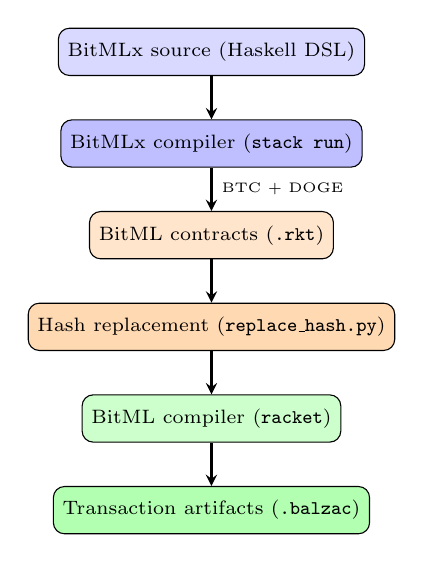
\begin{tikzpicture}[
    node distance=0.55cm,
    box/.style={rectangle, draw, rounded corners, minimum width=3.0cm, minimum height=0.6cm, font=\scriptsize, align=center},
    arr/.style={->, thick, >=stealth}
]
\node[box, fill=blue!15] (bitmlx) {BitMLx source (Haskell DSL)};
\node[box, fill=blue!25, below=of bitmlx] (compiler) {BitMLx compiler (\texttt{stack run})};
\node[box, fill=orange!20, below=of compiler] (rkt) {BitML contracts (\texttt{.rkt})};
\node[box, fill=orange!30, below=of rkt] (hash) {Hash replacement (\texttt{replace\_hash.py})};
\node[box, fill=green!20, below=of hash] (bitml) {BitML compiler (\texttt{racket})};
\node[box, fill=green!30, below=of bitml] (balzac) {Transaction artifacts (\texttt{.balzac})};
\draw[arr] (bitmlx) -- (compiler);
\draw[arr] (compiler) -- node[right, font=\tiny] {BTC + DOGE} (rkt);
\draw[arr] (rkt) -- (hash);
\draw[arr] (hash) -- (bitml);
\draw[arr] (bitml) -- (balzac);
\end{tikzpicture}
\caption{End-to-end compilation data flow, from a BitMLx specification to paired UTXO-level transaction artifacts. The compiler layer emits one \texttt{.rkt} program per chain; the pipeline layer then performs hash instantiation and Racket/Balzac lowering for each chain independently.}
\label{fig:pipeline}
\end{figure}

\begin{algorithm}[t]
\caption{BitMLx Compilation Pipeline}
\label{alg:pipeline}
\begin{algorithmic}[1]
\REQUIRE BitMLx example name $E$
\ENSURE Transaction artifacts for Bitcoin and Dogecoin
\STATE Initialize Docker container with Haskell, Racket, Python
\STATE Install BitML compiler as Racket package
\STATE Build BitMLx compiler via \texttt{stack build}
\STATE Execute \texttt{stack run -- $E$} to generate .rkt files
\FOR{each .rkt file $f$ in output directory}
    \STATE Replace hash placeholders with SHA-256 values
    \STATE Execute \texttt{racket $f$} to generate .balzac file
\ENDFOR
\STATE Compute statistics (transactions, depth, maximum timeout horizon)
\STATE Write results to \texttt{statistics.txt}
\end{algorithmic}
\end{algorithm}

Algorithm~\ref{alg:pipeline} describes the pipeline. The Docker container packages all dependencies: GHC and Stack for Haskell compilation, Racket for BitML compilation, and Python for hash replacement and statistics generation. Named Docker volumes cache compiled dependencies between runs.

\subsection{Integration Testing Framework}

The testing framework uses pytest to validate the pipeline end-to-end. Each test case executes the full compilation pipeline for a specific application and verifies:
\begin{itemize}
\item Existence of output files (.rkt, .balzac, depth) for both chains
\item Correctness of transaction counts via regex extraction
\item Correctness of execution tree depth values
\end{itemize}

\subsection{Web-Based Artifact Viewer}

The web application, built with Flask, provides three primary interfaces. The dashboard displays an overview of all compiled applications with comparative statistics rendered as CSS-based bar charts. The detail view presents the full artifacts for each application, including the Racket source, Balzac transactions, and compilation statistics. The interactive contract editor allows users to create contract variations by modifying participant names and deposit amounts for five available templates. The backend generates a temporary Haskell module, patches the example registry, executes the Docker pipeline, returns the compiled results, and restores the original source files in a \texttt{finally} block.

Security measures include input sanitization to prevent code injection into generated Haskell source and path traversal prevention when serving artifact files.

\section{Cross-Chain Application Design}

We evaluate the toolchain on four applications of increasing complexity, each demonstrating different BitMLx language features.

\subsection{ReceiverChosenDenomination}

This application models a cross-chain donation where the receiver chooses which denomination to accept. Participant $A$ deposits $(1~\text{BTC}, 1~\text{DOGE})$ and participant $B$ deposits nothing.

The contract offers $B$ three options via priority choice: (1) $B$ authorizes and receives 1~BTC while $A$ recovers 1~DOGE; (2) $B$ receives 1~DOGE while $A$ recovers 1~BTC; (3) all funds return to $A$ as a fallback. This application demonstrates the priority choice operator, authorization requirements, and fallback mechanisms.

\subsection{TwoPartyAgreement}

This application implements a secret-based agreement between two parties. Both participants commit secrets, and the contract outcome depends on the relationship between the revealed secret lengths.

Using \texttt{RevealIf} with predicate logic, the contract compares the lengths of secrets $a$ and $b$: if equal, funds are distributed according to one allocation; if different, an alternative allocation applies. This demonstrates the conditional revelation mechanism and predicate evaluation.

\subsection{MultichainPaymentExchange}

This application models a cross-chain payment through an exchange service involving three participants: a customer $C$ with 10~BTC, a receiver $R$, and an exchange $X$ with 100~DOGE. The contract enables $C$ to pay $R$ in BTC through $X$ at a fixed exchange rate, with fallback mechanisms ensuring no party loses funds if the exchange is not completed.

\subsection{MultichainLoanMediator}

The most complex application models a cross-chain loan with a mediator overseeing installment repayments. Borrower $B$ deposits 3~BTC as collateral, lender $L$ provides 30~DOGE, and mediator $M$ confirms each installment. The contract uses nested \texttt{Split} operations with multiple levels of authorization and priority choice, creating a deep execution tree where each repayment step requires mediator confirmation.

% Notation table moved to Section III

\section{Experimental Evaluation}

\subsection{Experimental Setup}

All reported artifact metrics were collected from the current repository state under \texttt{dist/bitmlx\_artifacts} and then cross-checked by redeploying the pipeline locally. The reproducible execution environment is defined by \texttt{docker/Dockerfile}, which uses Debian Bookworm, Stack 2.15.7, Racket, Python 3, and cached Docker volumes for Stack and Python dependencies. On the evaluation machine, the Docker image \texttt{blockchain-bitmlx:dev} was rebuilt successfully with host networking, the bootstrap step installed the BitML Racket package and built the Haskell executable, and \texttt{make test} completed all four pytest cases. Each application can be rebuilt independently with the pipeline described in Algorithm~\ref{alg:pipeline}. The ``timeout'' metric reported by the auxiliary statistics script is the largest \texttt{after} value found in the generated BitML/Racket contract; it is a protocol time horizon, not a wall-clock compilation time.

\subsection{Compilation Results}

Table~\ref{tab:results} presents the compilation results for all four applications.

\begin{table}[t]
\caption{Compilation results for the four cross-chain applications.}
\label{tab:results}
\centering
\footnotesize
\begin{tabular}{lccccc}
\toprule
Application & Part. & Secrets & Trans. & Depth & Timeout \\
\midrule
ReceiverChosenDenom. & 2 & 8 & 51 & 6 & 51 \\
TwoPartyAgreement & 2 & 10 & 51 & 6 & 51 \\
MultichainPayExch. & 3 & 12 & 207 & 9 & 51 \\
MultichainLoanMed. & 3 & 18 & 4098 & 27 & 61 \\
\bottomrule
\end{tabular}
\end{table}

The two-party applications (ReceiverChosenDenomination and TwoPartyAgreement) produce identical transaction counts of 51, despite TwoPartyAgreement requiring two additional secrets for the reveal-based predicates. The execution tree depth of 6 is consistent across both, reflecting their similar branching structure.

MultichainPaymentExchange, with three participants and an exchange intermediary, generates 207 transactions, a four-fold increase over the two-party cases. The additional participant introduces more step secrets and compensation branches, increasing the depth to 9.

MultichainLoanMediator exhibits dramatically higher complexity, producing 4,098 transactions with a depth of 27. The nested split operations and multiple mediator authorization steps create an exponential expansion in the transaction tree. Each installment step requires its own set of compensation branches, and the collateral mechanism for three participants further multiplies the output.

\subsection{Artifact Size Analysis}

Table~\ref{tab:artifacts} reports the artifact file sizes.

\begin{table}[t]
\caption{Artifact sizes in bytes for each application.}
\label{tab:artifacts}
\centering
\footnotesize
\begin{tabular}{lrrrr}
\toprule
Application & \begin{tabular}[c]{@{}r@{}}BTC\\(.rkt)\end{tabular} & \begin{tabular}[c]{@{}r@{}}DOGE\\(.rkt)\end{tabular} & \begin{tabular}[c]{@{}r@{}}BTC\\(.balzac)\end{tabular} & \begin{tabular}[c]{@{}r@{}}DOGE\\(.balzac)\end{tabular} \\
\midrule
RCD & 6,326 & 6,328 & 15,631 & 15,635 \\
TPA & 6,558 & 6,560 & 18,533 & 18,537 \\
MPE & 34,372 & 34,486 & 68,241 & 68,433 \\
MLM & 1,145,845 & 1,145,977 & 1,265,684 & 1,264,787 \\
\bottomrule
\end{tabular}
\end{table}

The Balzac artifacts are consistently larger than the corresponding Racket files by a factor of approximately 1.1x to 2.8x, reflecting the more verbose UTXO transaction descriptions. The difference between Bitcoin and Dogecoin artifacts for the same application is negligible (typically less than 0.5\%), confirming that the two chains share nearly identical transaction structures differing only in denomination labels.

MultichainLoanMediator produces over 1.1~MB of Racket code per chain, demonstrating that complex cross-chain contracts incur substantial artifact overhead.

\subsection{Complexity Scaling Analysis}

Fig.~\ref{fig:scaling} illustrates the relationship between contract structural features and compilation output.

\begin{figure}[t]
\centering
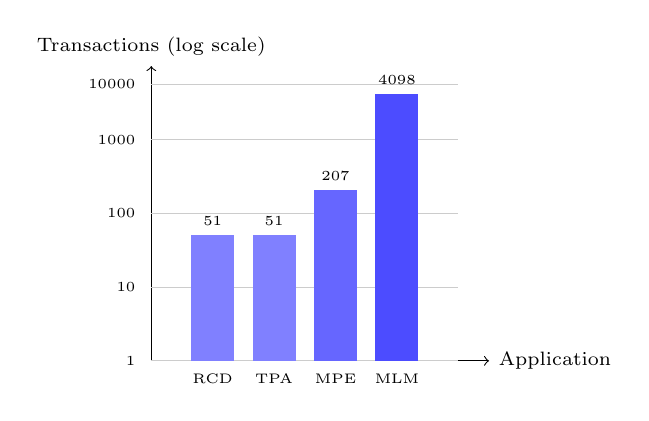
\begin{tikzpicture}[scale=0.78]
% Log-scale bar chart for transactions
\draw[->] (0,0) -- (5.5,0) node[right, font=\scriptsize] {Application};
\draw[->] (0,0) -- (0,4.8) node[above, font=\scriptsize] {Transactions (log scale)};
% Y-axis log ticks: 10, 100, 1000, 10000
\foreach \y/\val in {0/1, 1.2/10, 2.4/100, 3.6/1000} {
    \draw[gray!40] (0,\y) -- (5,\y);
    \node[font=\tiny, left] at (-0.1,\y) {\val};
}
\node[font=\tiny, left] at (-0.1,4.5) {10000};
\draw[gray!40] (0,4.5) -- (5,4.5);
% Bars (log10: 51→2.05, 207→2.78, 4098→4.34, scaled to fit)
\foreach \x/\label in {1/RCD, 2/TPA, 3/MPE, 4/MLM} {
    \node[font=\tiny] at (\x, -0.3) {\label};
}
\fill[blue!50] (0.65,0) rectangle (1.35,2.05);
\fill[blue!50] (1.65,0) rectangle (2.35,2.05);
\fill[blue!60] (2.65,0) rectangle (3.35,2.78);
\fill[blue!70] (3.65,0) rectangle (4.35,4.34);
\node[font=\tiny, above] at (1,2.05) {51};
\node[font=\tiny, above] at (2,2.05) {51};
\node[font=\tiny, above] at (3,2.78) {207};
\node[font=\tiny, above] at (4,4.34) {4098};
\end{tikzpicture}
\caption{Transaction count scaling across applications on a logarithmic scale. The 80x increase from two-party to three-party mediated contracts reveals the combinatorial expansion inherent in cross-chain compilation with nested control flow.}
\label{fig:scaling}
\end{figure}

The scaling behavior reveals three key observations. First, increasing the number of participants from 2 to 3 causes a superlinear increase in transactions due to additional compensation branches and collateral mechanisms. Second, nested control flow structures (splits within priority choices) cause exponential growth in the transaction tree. Third, the depth metric grows more moderately than the transaction count, indicating that the tree becomes wider rather than deeper as complexity increases.

\subsection{Compilation Performance}
\label{sec:compile-perf}

In addition to structural metrics, we measured the end-to-end wall-clock time of the compilation pipeline for each application. The measurement script \texttt{scripts/benchmark\_compile.sh} drives \texttt{scripts/bitmlx\_pipeline.sh} per application inside the \texttt{blockchain-bitmlx:dev} container with \texttt{BITMLX\_HASH\_SEED=42}, so that the seeded hash replacement (cf.\ Section~\ref{sec:reproducibility}) does not perturb timings between runs. Each measurement therefore captures the run of the pre-built Haskell executable via Stack, the BitMLx-to-BitML translation, the BitML-to-Balzac lowering in Racket, and the deterministic hash substitution. To account for run-to-run variability, each application is first executed once as a discarded warmup to stabilise the Stack and filesystem caches, after which five measured runs are timed using \texttt{date +\%s.\%N} and \texttt{awk}-based arithmetic. Table~\ref{tab:compile-time} reports the mean and sample standard deviation over the five runs, and Fig.~\ref{fig:compile-time} plots the mean against transaction count per chain with $\pm 1$ standard-deviation error bars.

\begin{table}[t]
\caption{End-to-end pipeline time per application, with seeded hashing (\texttt{BITMLX\_HASH\_SEED=42}). Mean and sample standard deviation over five measured runs (plus one discarded warmup), in seconds.}
\label{tab:compile-time}
\centering
\footnotesize
\begin{tabular}{lrr@{$\;\pm\;$}l}
\toprule
Application & Transactions per chain & \multicolumn{2}{c}{Wall-clock time (s)} \\
\midrule
ReceiverChosenDenom. & 51 & 3.086 & 0.156 \\
TwoPartyAgreement & 51 & 3.867 & 1.860 \\
MultichainPayExch. & 207 & 6.181 & 1.569 \\
MultichainLoanMed. & 4{,}098 & 107.461 & 3.447 \\
\bottomrule
\end{tabular}
\end{table}

\begin{figure}[t]
\centering
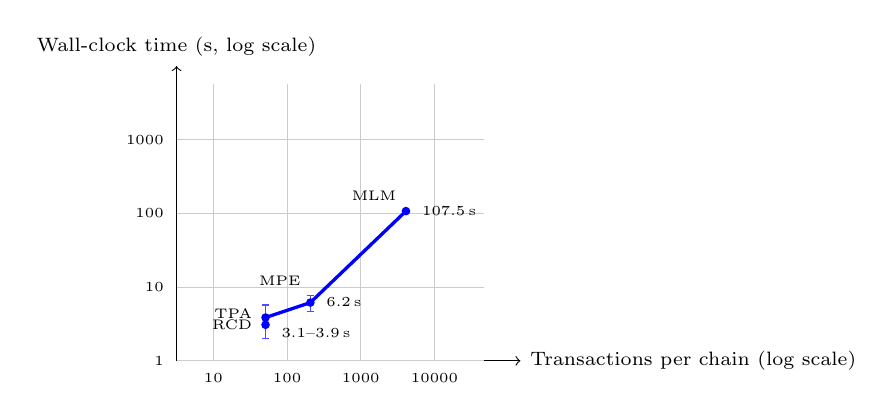
\begin{tikzpicture}[scale=0.78]
% Log-log line chart: x = 0.6 + 1.2*(log10(tx)-1), y = 1.2*log10(sec)
% Means over 5 runs: (51, 3.086), (51, 3.867), (207, 6.181), (4098, 107.461)
\draw[->] (0,0) -- (5.6,0) node[right, font=\scriptsize] {Transactions per chain (log scale)};
\draw[->] (0,0) -- (0,4.8) node[above, font=\scriptsize] {Wall-clock time (s, log scale)};
\foreach \x/\val in {0.6/10, 1.8/100, 3.0/1000, 4.2/10000} {
    \draw[gray!40] (\x,0) -- (\x,4.5);
    \node[font=\tiny, below] at (\x,-0.05) {\val};
}
\foreach \y/\val in {0/1, 1.2/10, 2.4/100, 3.6/1000} {
    \draw[gray!40] (0,\y) -- (5,\y);
    \node[font=\tiny, left] at (-0.05,\y) {\val};
}
% Mean points: RCD(1.449,0.587) TPA(1.449,0.705) MPE(2.179,0.949) MLM(3.735,2.438)
\draw[blue, very thick] (1.449,0.587) -- (1.449,0.705) -- (2.179,0.949) -- (3.735,2.438);
% +/-1 std-dev error bars (y converted via 1.2*log10):
% RCD [2.930,3.242]->[0.560,0.613]  TPA [2.007,5.727]->[0.363,0.910]
% MPE [4.612,7.750]->[0.797,1.067]  MLM [104.014,110.908]->[2.421,2.454]
\foreach \px/\lo/\hi in {1.449/0.560/0.613, 1.449/0.363/0.910, 2.179/0.797/1.067, 3.735/2.421/2.454} {
    \draw[blue!70] (\px,\lo) -- (\px,\hi);
    \draw[blue!70] (\px-0.06,\lo) -- (\px+0.06,\lo);
    \draw[blue!70] (\px-0.06,\hi) -- (\px+0.06,\hi);
}
\foreach \px/\py in {1.449/0.587, 1.449/0.705, 2.179/0.949, 3.735/2.438} {
    \fill[blue] (\px,\py) circle (2pt);
}
\node[font=\tiny, left] at (1.39,0.587) {RCD};
\node[font=\tiny, left] at (1.39,0.760) {TPA};
\node[font=\tiny, above left] at (2.179,1.067) {MPE};
\node[font=\tiny, above left] at (3.735,2.454) {MLM};
% Time annotations
\node[font=\tiny, right] at (1.55,0.45) {3.1--3.9\,s};
\node[font=\tiny, right] at (2.28,0.95) {6.2\,s};
\node[font=\tiny, right] at (3.84,2.44) {107.5\,s};
\end{tikzpicture}
\caption{Mean wall-clock compilation time versus transactions per chain, on log--log axes, with \texttt{BITMLX\_HASH\_SEED=42}. Markers show the mean of five measured runs and whiskers show $\pm 1$ sample standard deviation. The two-party contracts complete in a few seconds; their error bars overlap, so RCD and TPA are not reliably distinguishable at $51$ transactions. MultichainPaymentExchange remains in single-digit seconds, but the $80\times$ growth in transactions for MultichainLoanMediator translates into a $35\times$ increase in compile time, dominated by the Racket lowering and the hash-substitution pass over the multi-megabyte artifact.}
\label{fig:compile-time}
\end{figure}

The slope on the log--log plot becomes substantially steeper between MultichainPaymentExchange and MultichainLoanMediator, confirming that the runtime bottleneck is not the Haskell front end (which performs a single pass over a fixed BitMLx AST) but the downstream Racket lowering and the line-by-line hash substitution over the large generated \texttt{.rkt} and \texttt{.balzac} files. The variance is small relative to the mean for the dominant MultichainLoanMediator case (standard deviation $3.4$~s on a $107$~s mean, about $3\%$), whereas the two-party and three-party measurements show larger relative spread driven by occasional host-scheduling spikes during a run; the per-run figures are retained in the benchmark logs. This mirrors the transaction-tree expansion already visible in Fig.~\ref{fig:scaling} and identifies the lowering pass as the natural target for the compression strategies discussed in Section~\ref{sec:scalability}.

\subsection{Testing Verification}

All four applications pass the integration test suite, which verifies:
\begin{itemize}
\item Output file existence for both Bitcoin and Dogecoin chains
\item Transaction count matching: 51, 51, 207, and 4,098 respectively
\item Depth matching: 6, 6, 9, and 27 respectively
\end{itemize}

The test suite is intentionally metric-based: it checks exact transaction counts and depths, which remain stable even though the final hash literals are randomized by \texttt{replace\_hash.py}. This makes the tests robust to intended cryptographic placeholder replacement while still detecting structural regressions. In the local redeployment, \texttt{make test} rebuilt the Docker image, executed \texttt{scripts/bootstrap.sh}, and reported \texttt{4 passed} in $68.48$ seconds, with an end-to-end command elapsed time of $1$ minute $18.91$ seconds.

\subsection{Step Secret Generation Analysis}

Step secrets are central to BitMLx's cross-chain compensation mechanism. Each participant holds a unique secret at every node of the contract execution tree, with secret names encoding the L/R traversal path through priority choices and split branches. Table~\ref{tab:secrets} reports the number of step secrets generated per chain for each application, extracted by counting \texttt{secret} declarations in the compiled \texttt{.rkt} sources.

\begin{table}[t]
\caption{Step secret generation per application (Bitcoin chain).}
\label{tab:secrets}
\centering
\footnotesize
\begin{tabular}{lcccc}
\toprule
Application & Part. ($n$) & Depth ($d$) & Secrets ($S$) & $S/n$ \\
\midrule
RCD & 2 & 6 & 8 & 4.0 \\
TPA & 2 & 6 & 10 & 5.0 \\
MPE & 3 & 9 & 12 & 4.0 \\
MLM & 3 & 27 & 18 & 6.0 \\
\bottomrule
\end{tabular}
\end{table}

The number of step secrets correlates with both the depth of the priority-choice tree and the use of additional revelation primitives. TwoPartyAgreement requires two more secrets than ReceiverChosenDenomination despite identical depth, because its \texttt{RevealIf} clauses introduce additional commitments for the predicate-bound secrets. MultichainLoanMediator generates the highest absolute count due to its nested split structure, although its secrets-per-participant ratio (6.0) remains modest relative to its depth of 27. This indicates that BitMLx's secret generation scheme avoids the worst-case multiplicative blow-up that would result from instantiating independent secrets at every tree node, instead reusing the path-encoding scheme to share secrets along non-branching segments of the execution tree.

\subsection{Cross-Chain Structural Symmetry}

A central property of the BitMLx compilation strategy is that the Bitcoin and Dogecoin outputs share identical structure and differ only in coin denominations. We verified this property empirically by comparing the \texttt{<App>\_bitcoin.rkt} and \texttt{<App>\_dogecoin.rkt} files for each application after normalizing chain-specific identifiers.

For all four applications, the transaction counts and execution tree depths are identical between chains (cf.\ Table~\ref{tab:results}). The file size differences reported in Table~\ref{tab:artifacts} are small in relative terms (below $0.4\%$ in every case), attributable solely to differences in numeric coin values and chain labels rather than to structural divergence. The largest relative difference appears in MPE because DOGE literals ($100$) require more digits than BTC literals ($10$), while the largest absolute Balzac difference ($897$~bytes) occurs in MLM due to its much larger artifact size. No structural divergence was observed in any test, confirming that the two-pass compilation strategy with distinct \texttt{coinChooser} functions ($\mathit{fst}$ for Bitcoin, $\mathit{snd}$ for Dogecoin) correctly preserves the cross-chain symmetry mandated by the BitMLx semantics.

\subsection{Interactive Contract Editor Validation}

The web-based contract editor exposes five templates: SimpleExchange, ReceiverChosenDenomination, TwoPartyAgreement, MultichainPaymentExchange, and MultichainLoanMediator. Static inspection of \texttt{web/app.py} shows that the editor supports three implementation tasks: (1) read an existing Haskell template from \texttt{vendor/BitMLx/app/Examples}; (2) rewrite participant names, public keys, deposit declarations, and coin tuples; and (3) compile the temporary \texttt{UserCustom} example through the same Docker pipeline used by the command-line workflow.

Several safeguards are implemented. Participant names are restricted to alphanumeric characters and truncated to $20$ characters before insertion into generated Haskell source. Artifact file reads are constrained with \texttt{Path.resolve().is\_relative\_to(...)} to prevent path traversal. Temporary source changes are restored in a \texttt{finally} block after compilation, reducing the risk that a failed web request leaves \texttt{Main.hs} permanently modified. Invalid financial configurations are delegated to the BitMLx well-formedness checker, which can reject cases such as missing deposits, inconsistent withdrawals, or uncommitted secrets.

The redeployed web server was launched on \texttt{127.0.0.1:5002}. The dashboard, application-detail page, and Try Contract page all returned HTTP 200 responses. A live POST request to \texttt{/try/compile} using the SimpleExchange template with participants Alice and Bob completed successfully in $3.28$ seconds, generated the temporary \texttt{UserCustom} artifacts, and reported $31$ transactions, depth $4$, and timeout horizon $31$. This validates not only static artifact browsing but also the dynamic path from Flask input handling to Dockerized BitMLx compilation and Racket/Balzac generation.

This editor is therefore best understood as a safe, template-driven exploration interface rather than a full BitMLx visual programming environment. It lowers the barrier for non-Haskell users to inspect contract variations, while preserving the original compiler as the authoritative validator of semantic correctness.

\subsection{Metric Reproducibility and Hash Randomization}
\label{sec:reproducibility}

The compilation pipeline contains both deterministic and intentionally randomized components. The Haskell compiler deterministically generates the structural BitML/Racket contract from a fixed BitMLx source. The transaction count and execution-tree depth are therefore suitable regression metrics and are asserted exactly by the pytest suite. After Racket files are generated, \texttt{replace\_hash.py} replaces placeholder hashes with SHA-256 hashes of random strings, which by default makes byte-level checksums of final \texttt{.rkt} and \texttt{.balzac} artifacts non-identical across independent runs.

To enable byte-deterministic reviewer-side verification while preserving the original semantics, we extended \texttt{replace\_hash.py} with an explicit seeding interface. The script accepts an optional \texttt{--seed} argument and additionally honours the \texttt{BITMLX\_HASH\_SEED} environment variable; when either is set, the Python pseudo-random generator is reseeded before every line is processed, yielding identical hash literals on repeated executions of the same example. The unseeded code path is unchanged, so prior workflows that intentionally produce fresh secrets continue to do so. The benchmark script described in Section~\ref{sec:compile-perf} exports \texttt{BITMLX\_HASH\_SEED=42}, and a smoke test confirmed that two consecutive runs with the same seed produce byte-identical \texttt{.rkt} files for all four applications, while two unseeded runs differ exactly in the hash literals as expected. Reproducibility claims in this article are therefore at the level of structural metrics by default, and additionally at the byte level whenever the seed is supplied.

\section{Discussion}

\subsection{Transaction Overhead}

The most significant finding is the substantial transaction overhead inherent in the BitMLx compilation approach. Even a simple two-party donation requires 51 pre-signed transactions per chain, while a moderately complex loan protocol generates over 4,000. This overhead stems from the formal security model~\cite{engel2025bitmlx}: every possible execution path, including all compensation branches and collateral redistributions, must be pre-computed and encoded as transactions.

The protocol timeout horizon also increases for the most complex application, but this value should not be interpreted as wall-clock compiler runtime. In practice, most generated transactions will never be broadcast. An honest execution requires only a small subset of the pre-signed set. The remaining transactions serve as deterrents, ensuring that any deviation from the honest protocol can be countered by the injured party. This design mirrors the game-theoretic approach common in payment channel networks~\cite{gudgeon2020defi}, where the existence of punishment transactions ensures cooperative behavior.

\subsection{Comparison with HTLC-Based Approaches}

Traditional HTLC atomic swaps require only 4 transactions (2 per chain) for a two-party exchange, compared to the 51 generated by the BitMLx compilation. However, HTLCs support only simple exchanges and offer no mechanism for multi-step protocols, conditional branching, or mediated dispute resolution. The BitMLx approach trades transaction efficiency for expressiveness and formal security guarantees.

\subsection{Scalability Considerations}
\label{sec:scalability}

The exponential growth observed in MultichainLoanMediator raises concerns about the scalability of the approach to more complex contracts. Possible mitigation strategies include: (1) compilation optimizations that identify and merge equivalent transaction subtrees; (2) off-chain execution of compensation logic, broadcasting only the minimal required transactions; and (3) layered contract designs that decompose complex protocols into simpler sub-protocols.

Notably, the step secret count grows much more moderately than the transaction count: while transactions increase from $51$ to $4{,}098$ (a factor of $80\times$) across the test applications, secret counts increase only from $8$ to $18$ (a factor of $2.25\times$). This sublinear growth confirms that the path-encoding scheme used by \texttt{StepSecrets.hs} effectively shares secrets across non-branching segments of the execution tree, avoiding the multiplicative blow-up that a naive node-by-node assignment would induce. The bottleneck for cross-chain compilation thus lies in the transaction tree expansion rather than in the cryptographic commitment overhead.

\subsection{Compressing Compensation Branches with MAST on Taproot}
\label{sec:mast}

A more aggressive on-chain mitigation, presented here as a theoretical proposal rather than an implemented feature, is to compress unused compensation branches into Merkleized Abstract Syntax Trees (MAST) carried by Bitcoin Taproot outputs~\cite{nick2020bip341,wuille2020bip342}. The empirical results in Table~\ref{tab:results} show that every BitMLx compilation enumerates the full set of pre-signed transactions for every honest and adversarial branch, even though in any single execution only one root-to-leaf path is ever broadcast. Pre-Taproot Bitcoin Script forces all alternative spending conditions to live inline in the output script, which is why the BitMLx lowering currently materialises one explicit transaction per branch.

Taproot replaces this inline encoding with a tree of script leaves whose root is committed to via a Merkle root mixed into the output public key. To spend the output, the redeemer only needs to reveal (i) the leaf script actually used, (ii) the Merkle path proving its inclusion, and (iii) the internal key. Unused leaves are never published on-chain, so their cost is amortised away.

Applied to the BitMLx execution tree, the proposal is as follows. The set of pre-signed transactions emitted at a single contract state (the stipulation node, a priority-choice node, or a split node) shares a common funding output. Today each branch consumes that output through its own distinct \texttt{transaction} declaration. Under a MAST encoding, each branch would become one leaf of a Tapscript tree rooted at the funding output's Taproot key:
\begin{itemize}
\item the \emph{honest-path} leaf, signed by the legitimate next participant according to the priority order;
\item one \emph{compensation} leaf per losing branch, encoding the punishment or refund condition currently materialised as a dedicated pre-signed transaction;
\item the \emph{timeout / collateral-recovery} leaves implementing the \texttt{after}-clauses.
\end{itemize}
Because every losing branch in the BitMLx execution model has the same parent state, this transformation is purely local: it does not alter the global tree of states, only how the alternatives at one state are encoded into the output script. The cross-chain semantics is preserved as long as Dogecoin retains an equivalent encoding; in practice this means MAST compression is asymmetric and could be enabled on Bitcoin alone while Dogecoin continues to use the existing inline lowering, since BitMLx already tolerates per-chain coin-selection differences and the well-formedness check operates on the structural metrics rather than on the script encoding.

The expected on-chain footprint reduction is asymmetric in the same way that the cost of pre-signed compensation transactions is asymmetric: an honest execution pays only the Merkle path overhead ($\log_2 k$ hashes, where $k$ is the branching factor at the current state) plus the single leaf script, instead of carrying the full inline script enumerating all $k$ branches. For MultichainLoanMediator, whose contract repeatedly branches at every installment step, the dominant compensation leaves never reach the chain, so the practical on-chain cost of an honest repayment becomes essentially independent of the depth of the punishment tree --- mirroring the well-known argument for Taproot-based Lightning channels~\cite{poon2016bitcoin}. The complication is that BitMLx security proofs are written against the BitML transaction-level semantics: a future article would need to lift the soundness argument of~\cite{engel2025bitmlx} to a MAST-extended target language, showing that revealing only the executed leaf does not weaken the honest-strategy guarantees. This article identifies the opportunity and the engineering shape of the modification; the formal lifting and a prototype Taproot back end are left as future work.

\subsection{Validation Through Symmetry and Determinism}

The empirical verification of cross-chain structural symmetry, with small relative size deviations between Bitcoin and Dogecoin outputs across all four applications, provides an additional correctness check beyond the integration test suite. Any divergence in the structure of the two outputs would indicate a bug in the coin-selection logic or in the shared compilation passes; the observed equality across all tests increases confidence in the implementation. Likewise, the determinism of \texttt{.rkt} generation enables byte-level regression detection, complementing the value-based assertions of the pytest suite.

\subsection{Toolchain Reproducibility}

The Docker-based containerization ensures complete reproducibility of the compilation environment. All dependencies, including Stack, Racket, Python, LLVM, and C build tools, are installed in the Docker image, while named Docker volumes cache the Stack toolchain and Python virtual environment between runs. The Makefile provides simple entry points for common operations, lowering the barrier to replication. The redeployment also exposed a practical systems issue: some laboratory Docker installations may not provide the default bridge network. The updated wrapper detects this condition and uses host networking so that the scientific result remains reproducible on the available machine.

\subsection{Path Toward Testnet Deployment}
\label{sec:testnet}

The artifacts evaluated in this article are validated structurally through the integration test suite and by direct inspection of the compiled \texttt{.rkt} and \texttt{.balzac} files; they have not yet been broadcast to any live network. The Balzac descriptions are nevertheless designed to be directly compilable to standard UTXO transactions, so on-chain execution validation is the natural next step. We outline the methodology rather than reporting fabricated on-chain numbers, in order to keep the empirical claims of this article faithful to what was actually observed on the evaluation machine.

A minimal end-to-end testnet experiment for the simplest application, ReceiverChosenDenomination, would proceed as follows. The Balzac stipulation transaction and a single honest-path branch (one priority choice, one withdraw) would be lowered to Bitcoin Testnet and Dogecoin Testnet transactions, funded from public faucet outputs at both endpoints. Reasonable parameter choices, given typical Testnet conditions, are: a fee target around $1$~sat/vB for Bitcoin Testnet and the analogous minimum relay fee for Dogecoin Testnet; dust limits of $546$~satoshi for Bitcoin and the Dogecoin-default $0.01$~DOGE; opt-in Replace-By-Fee enabled at the funding step so that the experiment can be retried at higher fees if a Testnet node refuses to relay; and a conservative confirmation target of at least one Bitcoin block (Testnet block intervals are highly variable but average around ten minutes) and six Dogecoin blocks (each averaging one minute). The honest-path branch involves a single stipulation transaction per chain plus the chosen withdraw transaction, so the total on-chain footprint is bounded by the transaction-tree leaf count along the executed path rather than by the full count in Table~\ref{tab:results}. To make the resulting numbers reviewer-verifiable, the experiment would record, for each broadcast transaction, the Testnet transaction identifier, the raw virtual size in bytes, the actual fee paid in satoshi (respectively koinu), and the block height at which it confirmed; these per-transaction rows would form a new table appended to the Experimental Evaluation section in a follow-up article.

The reason this experiment is not run here is that it requires coordination outside the scope of an automated reproducibility build: Testnet coin faucets are rate-limited and require external requests, and live broadcasts cannot be re-run hermetically inside the Docker harness used for the redeployment in this article. The methodology above is included so that the testnet step can be carried out and reported in a subsequent article without redesigning the toolchain; the compiler back end already emits the standard Balzac transactions that such an experiment requires.

\subsection{Limitations}

The current implementation has several limitations. First, only Bitcoin and Dogecoin are supported as target chains; extending to other UTXO-based chains requires adding new coin selectors and chain-specific configurations. Second, the compiled transactions have been validated structurally and verified to load through the Balzac description format, but have not yet been broadcast to any testnet or mainnet; Section~\ref{sec:testnet} describes the methodology for that follow-up step. Third, the web-based contract editor supports only template-based modifications rather than arbitrary contract construction. Fourth, large contracts such as MultichainLoanMediator generate megabyte-scale artifacts and thousands of transaction templates, which may be cumbersome for interactive inspection even when the command-line pipeline completes successfully.

\section{Data and Code Availability}
\label{sec:availability}

The complete source code of the toolchain, the four worked example contracts, the Docker build files, the integration test suite, the Flask web application, the deterministic hash-replacement script described in Section~\ref{sec:reproducibility}, and the wall-clock benchmark script used to produce Table~\ref{tab:compile-time} and Fig.~\ref{fig:compile-time} are publicly available at \url{https://github.com/sampleit533/BitMLx/}. Byte-deterministic regeneration of the artifacts evaluated in Section~VI requires only running \texttt{scripts/benchmark\_compile.sh} inside the \texttt{blockchain-bitmlx:dev} container with the default \texttt{BITMLX\_HASH\_SEED=42} environment variable. Pre-built artifacts for the four applications are committed under \texttt{dist/bitmlx\_artifacts/} for reviewers who prefer to inspect the outputs without rebuilding.

\section{Conclusion}

This article has presented a comprehensive toolchain for compiling, testing, and visualizing cross-chain smart contracts based on the BitMLx domain-specific language. The system integrates a Haskell-based compiler, a Docker-containerized build pipeline, a pytest-based testing framework, and a Flask-based web application into a cohesive platform for cross-chain contract development.

Evaluation on four representative applications demonstrated the toolchain's ability to handle contracts of varying complexity, from simple two-party donations to complex mediated loan protocols. The results quantified the relationship between contract structure and compilation output, revealing that transaction counts grow sharply with nested control flow structures (from $51$ to $4{,}098$ transactions) while step-secret counts grow more moderately (from $8$ to $18$). The wall-clock benchmark reported in Table~\ref{tab:compile-time}, averaged over five runs, further showed that the end-to-end pipeline completes in a few seconds for the two-party applications ($3.1$ and $3.9$~s on average), in about six seconds for the three-party MultichainPaymentExchange, and in roughly $107$~seconds for MultichainLoanMediator, identifying the Racket lowering and the hash-substitution pass as the dominant cost on the largest contract. Cross-chain structural symmetry was observed through identical transaction counts and depths for Bitcoin and Dogecoin outputs, with file-size differences attributable to denomination labels and numeric literals. The pytest suite confirms the expected structural metrics for all four evaluated applications, and the Flask editor extends the toolchain with a template-driven interactive interface. As part of this article, the hash-replacement script was extended with explicit seed support (Section~\ref{sec:reproducibility}), so reviewers can regenerate byte-identical artifacts via \texttt{BITMLX\_HASH\_SEED}.

Future work includes extending the compiler to support additional UTXO-based blockchains, implementing compilation optimizations to reduce transaction overhead --- in particular a Taproot-based back end that compresses unused compensation branches into MAST script trees as outlined in Section~\ref{sec:mast} ---, deploying compiled contracts to Bitcoin Testnet and Dogecoin Testnet following the methodology of Section~\ref{sec:testnet} for on-chain validation with measured fees and confirmation times, and developing a visual contract designer that enables users to construct arbitrary cross-chain protocols without writing Haskell code.

\begin{thebibliography}{99}

\bibitem{bartoletti2018bitml}
M.~Bartoletti and R.~Zunino, ``BitML: A calculus for Bitcoin smart contracts,'' in \textit{Proc. ACM SIGSAC Conf. Comput. Commun. Secur. (CCS)}, Toronto, ON, Canada, 2018, pp.~83--100.

\bibitem{bartoletti2019bitml}
M.~Bartoletti and R.~Zunino, ``Verifying liquidity of Bitcoin contracts,'' in \textit{Proc. Int. Conf. Principles Secur. Trust (POST)}, Prague, Czech Republic, 2019, pp.~222--243.

\bibitem{engel2025bitmlx}
S.~Engel and M.~Maffei, ``BitMLx: Cross-chain smart contracts for Bitcoin-style blockchains,'' arXiv preprint arXiv:2501.17733, Jan. 2025.

\bibitem{herlihy2018atomic}
M.~Herlihy, ``Atomic cross-chain swaps,'' in \textit{Proc. ACM Symp. Principles Distrib. Comput. (PODC)}, Egham, UK, 2018, pp.~245--254.

\bibitem{thyagarajan2022universal}
S.~A.~K.~Thyagarajan, G.~Malavolta, and P.~Moreno-Sanchez, ``Universal atomic swaps: Secure exchange of coins across all blockchains,'' in \textit{Proc. IEEE Symp. Secur. Privacy (S\&P)}, San Francisco, CA, USA, 2022, pp.~1299--1316.

\bibitem{han2019threshold}
R.~Han, H.~Lin, and J.~Yu, ``On the optionality and fairness of atomic swaps,'' in \textit{Proc. ACM Conf. Adv. Financial Technol. (AFT)}, Zurich, Switzerland, 2021, pp.~62--75.

\bibitem{xie2022bridge}
T.~Xie, J.~Zhang, Z.~Cheng, F.~Zhang, Y.~Zhang, Y.~Jia, D.~Boneh, and D.~Song, ``zkBridge: Trustless cross-chain bridges made practical,'' in \textit{Proc. ACM SIGSAC Conf. Comput. Commun. Secur. (CCS)}, Los Angeles, CA, USA, 2022, pp.~3003--3017.

\bibitem{belchior2021survey}
R.~Belchior, A.~Vasconcelos, S.~Guerreiro, and M.~Correia, ``A survey on blockchain interoperability: Past, present, and future trends,'' \textit{ACM Comput. Surv.}, vol.~54, no.~8, pp.~1--41, Nov. 2022.

\bibitem{atzei2019developing}
N.~Atzei, M.~Bartoletti, T.~Cimoli, S.~Lande, and R.~Zunino, ``Developing secure Bitcoin contracts with BitML,'' in \textit{Proc. Eur. Symp. Secur. Privacy Workshops (EuroS\&PW)}, Stockholm, Sweden, 2019, pp.~208--213.

\bibitem{bartoletti2025comparison}
M.~Bartoletti, ``A comparison of smart contract languages and platforms,'' \textit{Future Gener. Comput. Syst.}, vol.~164, Art. no.~107540, Mar. 2025.

\bibitem{bonneau2015sok}
J.~Bonneau, A.~Miller, J.~Clark, A.~Narayanan, J.~A.~Kroll, and E.~W.~Felten, ``SoK: Research perspectives and challenges for Bitcoin and cryptocurrencies,'' in \textit{Proc. IEEE Symp. Secur. Privacy (S\&P)}, San Jose, CA, USA, 2015, pp.~104--121.

\bibitem{zamyatin2021sok}
A.~Zamyatin, M.~Al-Bassam, D.~Zindros, E.~Kokoris-Kogias, P.~Moreno-Sanchez, A.~Kiayias, and W.~J.~Knottenbelt, ``SoK: Communication across distributed ledgers,'' in \textit{Proc. Financial Cryptogr. Data Secur. (FC)}, Virtual, 2021, pp.~3--36.


\bibitem{nakamoto2008bitcoin}
S.~Nakamoto, ``Bitcoin: A peer-to-peer electronic cash system,'' White paper, 2008.

\bibitem{wood2014ethereum}
G.~Wood, ``Ethereum: A secure decentralised generalised transaction ledger,'' \textit{Ethereum Project Yellow Paper}, vol.~151, pp.~1--32, 2014.

\bibitem{amsden2020move}
Z.~Amsden \textit{et al.}, ``The Libra blockchain,'' White paper, 2019.

\bibitem{sergey2019scilla}
I.~Sergey, V.~Nagaraj, J.~Johannsen, A.~Kumar, A.~Trunov, and K.~Chan, ``Safer smart contract programming with Scilla,'' \textit{Proc. ACM Program. Lang.}, vol.~3, no.~OOPSLA, Art. no.~185, Oct. 2019.

\bibitem{kwon2019cosmos}
J.~Kwon and E.~Buchman, ``Cosmos whitepaper: A network of distributed ledgers,'' White paper, 2019.

\bibitem{wood2016polkadot}
G.~Wood, ``Polkadot: Vision for a heterogeneous multi-chain framework,'' White paper, 2016.

\bibitem{gudgeon2020defi}
L.~Gudgeon, P.~Moreno-Sanchez, S.~Perez-Sola, B.~Livshits, and A.~Gervais, ``SoK: Layer-two blockchain protocols,'' in \textit{Proc. Financial Cryptogr. Data Secur. (FC)}, Kota Kinabalu, Malaysia, 2020, pp.~201--226.

\bibitem{tikhomirov2018smartcheck}
S.~Tikhomirov, E.~Voskresenskaya, I.~Ivanitskiy, R.~Takhaviev, E.~Marchenko, and Y.~Alexandrov, ``SmartCheck: Static analysis of Ethereum smart contracts,'' in \textit{Proc. ACM/IEEE Int. Workshop Emerg. Trends Softw. Eng. Blockchain (WETSEB)}, Gothenburg, Sweden, 2018, pp.~9--16.

\bibitem{nick2020bip341}
P.~Wuille, J.~Nick, and A.~Towns, ``Taproot: SegWit version~1 spending rules,'' Bitcoin Improvement Proposal BIP~341, Jan. 2020.

\bibitem{wuille2020bip342}
P.~Wuille, J.~Nick, and A.~Towns, ``Validation of Taproot scripts,'' Bitcoin Improvement Proposal BIP~342, Jan. 2020.

\bibitem{poon2016bitcoin}
J.~Poon and T.~Dryja, ``The Bitcoin Lightning Network: Scalable off-chain instant payments,'' White paper, Jan. 2016.

\end{thebibliography}

\end{document}
